\documentclass[tikz,border=15pt]{standalone}
\usepackage{tikz}
\usepackage{xcolor}
\usetikzlibrary{arrows.meta,calc,patterns}

\definecolor{bgcolor}{RGB}{15,23,42}
\definecolor{cardbg}{RGB}{30,41,59}
\definecolor{cardborder}{RGB}{51,65,85}
\definecolor{fluidhigh}{RGB}{2,132,199}
\definecolor{fluidlow}{RGB}{245,158,11}
\definecolor{cyanhigh}{RGB}{56,189,248}
\definecolor{amberlow}{RGB}{251,191,36}
\definecolor{metalgray}{RGB}{148,163,184}
\definecolor{metalhatch}{RGB}{100,116,139}
\definecolor{rodcolor}{RGB}{226,232,240}
\definecolor{sealred}{RGB}{239,68,68}
\definecolor{greendrive}{RGB}{34,197,94}
\definecolor{greenbg}{RGB}{20,83,45}
\definecolor{greentext}{RGB}{74,222,128}
\definecolor{inletbg}{RGB}{12,74,110}
\definecolor{outletbg}{RGB}{113,63,18}
\definecolor{sealtext}{RGB}{248,113,113}

\begin{document}
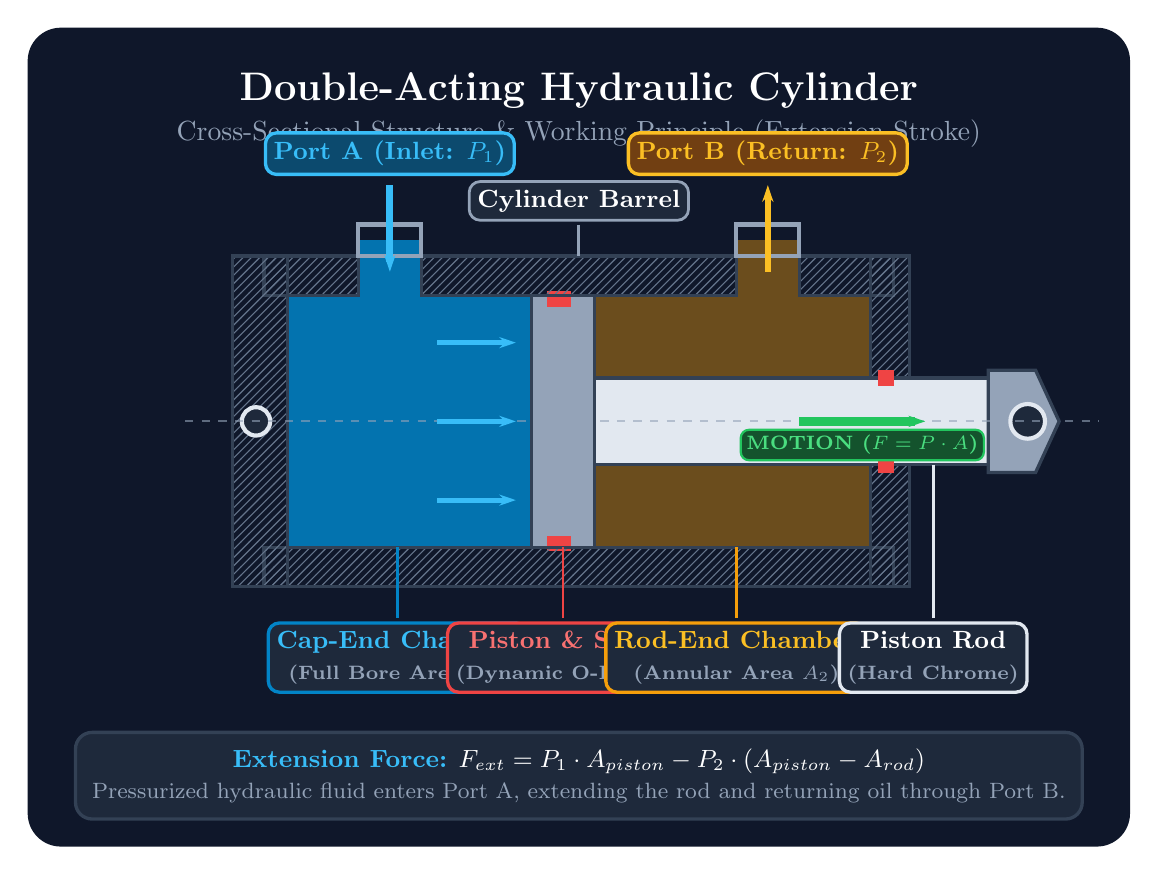
\begin{tikzpicture}[
    >={Stealth[length=6pt, width=4pt]}
]

% Background Card
\fill[rounded corners=12pt, fill=bgcolor] (-7.0,-5.2) rectangle (7.0,5.2);

% Title & Header
\node[text=white, font=\Large\bfseries] at (0, 4.4) {Double-Acting Hydraulic Cylinder};
\node[text=metalgray, font=\normalsize] at (0, 3.85) {Cross-Sectional Structure \& Working Principle (Extension Stroke)};

% Base Origin inside Cylinder: center of bore at (0, 0.2)
\coordinate (C) at (0, 0.2);

% Dimensions
% Bore radius = 1.6, Total barrel length = 8.0 (-4.0 to +4.0)
% Piston width = 0.8 (-0.6 to +0.2), Rod radius = 0.55, Rod length = 5.2 (+0.2 to +5.4)

% 1. FLUID VOLUMES
% Cap-End Chamber (High Pressure Blue)
\fill[fluidhigh, opacity=0.85] (-3.7, -1.4) rectangle (-0.6, 1.8);
% Rod-End Chamber (Low Pressure Amber)
\fill[fluidlow, opacity=0.4] (0.2, -1.4) rectangle (3.7, 1.8);

% Inflow & Outflow Port Volumes
\fill[fluidhigh, opacity=0.85] (-2.8, 1.8) rectangle (-2.0, 2.5);
\fill[fluidlow, opacity=0.4] (2.0, 1.8) rectangle (2.8, 2.5);

% 2. PISTON & STEEL ROD
% Hard Chrome Rod
\fill[rodcolor, draw=cardborder, line width=1.2pt] (0.2, -0.35) rectangle (5.2, 0.75);
% Clevis Rod End
\fill[fill=metalgray, draw=cardborder, line width=1.2pt] (5.2, -0.45) -- (5.8, -0.45) -- (6.1, 0.2) -- (5.8, 0.85) -- (5.2, 0.85) -- cycle;
\fill[fill=cardbg, draw=rodcolor, line width=1.5pt] (5.7, 0.2) circle (0.22cm);

% Piston Body
\fill[metalgray, draw=cardborder, line width=1.2pt] (-0.6, -1.4) rectangle (0.2, 1.8);
% Dynamic Seals
\fill[sealred] (-0.4, 1.65) rectangle (-0.1, 1.85);
\fill[sealred] (-0.4, -1.45) rectangle (-0.1, -1.25);

% 3. BARREL WALLS & GLAND (Hatched Metal)
% Top barrel wall
\fill[pattern=north east lines, pattern color=metalhatch, draw=cardborder, line width=1.2pt]
    (-4.0, 1.8) -- (-2.8, 1.8) -- (-2.8, 2.3) -- (-2.0, 2.3) -- (-2.0, 1.8) --
    (2.0, 1.8) -- (2.0, 2.3) -- (2.8, 2.3) -- (2.8, 1.8) -- (4.0, 1.8) --
    (4.0, 2.3) -- (-4.0, 2.3) -- cycle;

% Bottom barrel wall
\fill[pattern=north east lines, pattern color=metalhatch, draw=cardborder, line width=1.2pt] (-4.0, -1.9) rectangle (4.0, -1.4);

% Cap End (Left Blind End)
\fill[pattern=north east lines, pattern color=metalhatch, draw=cardborder, line width=1.2pt] (-4.4, -1.9) rectangle (-3.7, 2.3);
\fill[fill=cardbg, draw=rodcolor, line width=1.5pt] (-4.1, 0.2) circle (0.18cm);

% Rod Gland End (Right)
\fill[pattern=north east lines, pattern color=metalhatch, draw=cardborder, line width=1.2pt] (3.7, 0.75) rectangle (4.2, 2.3);
\fill[pattern=north east lines, pattern color=metalhatch, draw=cardborder, line width=1.2pt] (3.7, -1.9) rectangle (4.2, -0.35);
% Rod seals
\fill[sealred] (3.8, 0.65) rectangle (4.0, 0.85);
\fill[sealred] (3.8, -0.45) rectangle (4.0, -0.25);

% Port Pipes
\draw[metalgray, line width=1.5pt] (-2.8, 2.3) rectangle (-2.0, 2.7);
\draw[metalgray, line width=1.5pt] (2.0, 2.3) rectangle (2.8, 2.7);

% Center Axis Line
\draw[metalgray, dashed, line width=0.8pt, opacity=0.6] (-5.0, 0.2) -- (6.6, 0.2);

% 4. FLOW ARROWS & MOTION
% Inflow arrows
\draw[cyanhigh, line width=2.5pt, ->] (-2.4, 3.2) -- (-2.4, 2.1);
\draw[cyanhigh, line width=1.8pt, ->] (-1.8, 1.2) -- (-0.8, 1.2);
\draw[cyanhigh, line width=1.8pt, ->] (-1.8, 0.2) -- (-0.8, 0.2);
\draw[cyanhigh, line width=1.8pt, ->] (-1.8, -0.8) -- (-0.8, -0.8);

% Outflow arrows
\draw[amberlow, line width=2.0pt, ->] (2.4, 2.1) -- (2.4, 3.2);

% Motion Arrow
\draw[greendrive, line width=3.5pt, ->] (2.8, 0.2) -- (4.4, 0.2);
\node[fill=greenbg, draw=greendrive, line width=0.8pt, rounded corners=3pt, text=greentext, font=\scriptsize\bfseries, inner sep=2pt] at (3.6, -0.1) {MOTION ($F = P\cdot A$)};

% 5. LABELS & CALLOUTS
% Port A
\node[fill=inletbg, draw=cyanhigh, line width=1.2pt, rounded corners=4pt, text=cyanhigh, font=\small\bfseries, inner sep=3pt] at (-2.4, 3.6) {Port A (Inlet: $P_1$)};
% Port B
\node[fill=outletbg, draw=amberlow, line width=1.2pt, rounded corners=4pt, text=amberlow, font=\small\bfseries, inner sep=3pt] at (2.4, 3.6) {Port B (Return: $P_2$)};

% Barrel Label
\node[fill=cardbg, draw=metalgray, line width=1pt, rounded corners=4pt, text=white, font=\small\bfseries, inner sep=3pt] at (0, 3.0) {Cylinder Barrel};
\draw[metalgray, line width=1pt] (0, 2.7) -- (0, 2.3);

% Bottom Labels
% Cap-End Chamber
\node[fill=cardbg, draw=fluidhigh, line width=1.2pt, rounded corners=4pt, text=cyanhigh, font=\small\bfseries, align=center, inner sep=3pt] at (-2.3, -2.8) {Cap-End Chamber\\\textcolor{metalgray}{\scriptsize (Full Bore Area $A_1$)}};
\draw[fluidhigh, line width=1pt] (-2.3, -2.3) -- (-2.3, -1.4);

% Piston & Seals
\node[fill=cardbg, draw=sealred, line width=1.2pt, rounded corners=4pt, text=sealtext, font=\small\bfseries, align=center, inner sep=3pt] at (-0.2, -2.8) {Piston \& Seals\\\textcolor{metalgray}{\scriptsize (Dynamic O-Rings)}};
\draw[sealred, line width=1pt] (-0.2, -2.3) -- (-0.2, -1.4);

% Rod-End Chamber
\node[fill=cardbg, draw=fluidlow, line width=1.2pt, rounded corners=4pt, text=amberlow, font=\small\bfseries, align=center, inner sep=3pt] at (2.0, -2.8) {Rod-End Chamber\\\textcolor{metalgray}{\scriptsize (Annular Area $A_2$)}};
\draw[fluidlow, line width=1pt] (2.0, -2.3) -- (2.0, -1.4);

% Piston Rod
\node[fill=cardbg, draw=rodcolor, line width=1.2pt, rounded corners=4pt, text=white, font=\small\bfseries, align=center, inner sep=3pt] at (4.5, -2.8) {Piston Rod\\\textcolor{metalgray}{\scriptsize (Hard Chrome)}};
\draw[rodcolor, line width=1pt] (4.5, -2.3) -- (4.5, -0.35);

% Summary Card (Bottom)
\node[fill=cardbg, draw=cardborder, line width=1.2pt, rounded corners=6pt, text=white, font=\small, align=center, inner sep=6pt] at (0, -4.3) {
    \textbf{\textcolor{cyanhigh}{Extension Force:}} $F_{ext} = P_1 \cdot A_{piston} - P_2 \cdot (A_{piston} - A_{rod})$\\
    \textcolor{metalgray}{\footnotesize Pressurized hydraulic fluid enters Port A, extending the rod and returning oil through Port B.}
};

\end{tikzpicture}
\end{document}
